% Options for packages loaded elsewhere
\PassOptionsToPackage{unicode}{hyperref}
\PassOptionsToPackage{hyphens}{url}
\PassOptionsToPackage{dvipsnames,svgnames,x11names}{xcolor}
%
\documentclass[
]{article}

\usepackage{amsmath,amssymb}
\usepackage{iftex}
\ifPDFTeX
  \usepackage[T1]{fontenc}
  \usepackage[utf8]{inputenc}
  \usepackage{textcomp} % provide euro and other symbols
\else % if luatex or xetex
  \usepackage{unicode-math}
  \defaultfontfeatures{Scale=MatchLowercase}
  \defaultfontfeatures[\rmfamily]{Ligatures=TeX,Scale=1}
\fi
\usepackage{lmodern}
\ifPDFTeX\else  
    % xetex/luatex font selection
\fi
% Use upquote if available, for straight quotes in verbatim environments
\IfFileExists{upquote.sty}{\usepackage{upquote}}{}
\IfFileExists{microtype.sty}{% use microtype if available
  \usepackage[]{microtype}
  \UseMicrotypeSet[protrusion]{basicmath} % disable protrusion for tt fonts
}{}
\makeatletter
\@ifundefined{KOMAClassName}{% if non-KOMA class
  \IfFileExists{parskip.sty}{%
    \usepackage{parskip}
  }{% else
    \setlength{\parindent}{0pt}
    \setlength{\parskip}{6pt plus 2pt minus 1pt}}
}{% if KOMA class
  \KOMAoptions{parskip=half}}
\makeatother
\usepackage{xcolor}
\setlength{\emergencystretch}{3em} % prevent overfull lines
\setcounter{secnumdepth}{5}
% Make \paragraph and \subparagraph free-standing
\makeatletter
\ifx\paragraph\undefined\else
  \let\oldparagraph\paragraph
  \renewcommand{\paragraph}{
    \@ifstar
      \xxxParagraphStar
      \xxxParagraphNoStar
  }
  \newcommand{\xxxParagraphStar}[1]{\oldparagraph*{#1}\mbox{}}
  \newcommand{\xxxParagraphNoStar}[1]{\oldparagraph{#1}\mbox{}}
\fi
\ifx\subparagraph\undefined\else
  \let\oldsubparagraph\subparagraph
  \renewcommand{\subparagraph}{
    \@ifstar
      \xxxSubParagraphStar
      \xxxSubParagraphNoStar
  }
  \newcommand{\xxxSubParagraphStar}[1]{\oldsubparagraph*{#1}\mbox{}}
  \newcommand{\xxxSubParagraphNoStar}[1]{\oldsubparagraph{#1}\mbox{}}
\fi
\makeatother

\usepackage{color}
\usepackage{fancyvrb}
\newcommand{\VerbBar}{|}
\newcommand{\VERB}{\Verb[commandchars=\\\{\}]}
\DefineVerbatimEnvironment{Highlighting}{Verbatim}{commandchars=\\\{\}}
% Add ',fontsize=\small' for more characters per line
\usepackage{framed}
\definecolor{shadecolor}{RGB}{241,243,245}
\newenvironment{Shaded}{\begin{snugshade}}{\end{snugshade}}
\newcommand{\AlertTok}[1]{\textcolor[rgb]{0.68,0.00,0.00}{#1}}
\newcommand{\AnnotationTok}[1]{\textcolor[rgb]{0.37,0.37,0.37}{#1}}
\newcommand{\AttributeTok}[1]{\textcolor[rgb]{0.40,0.45,0.13}{#1}}
\newcommand{\BaseNTok}[1]{\textcolor[rgb]{0.68,0.00,0.00}{#1}}
\newcommand{\BuiltInTok}[1]{\textcolor[rgb]{0.00,0.23,0.31}{#1}}
\newcommand{\CharTok}[1]{\textcolor[rgb]{0.13,0.47,0.30}{#1}}
\newcommand{\CommentTok}[1]{\textcolor[rgb]{0.37,0.37,0.37}{#1}}
\newcommand{\CommentVarTok}[1]{\textcolor[rgb]{0.37,0.37,0.37}{\textit{#1}}}
\newcommand{\ConstantTok}[1]{\textcolor[rgb]{0.56,0.35,0.01}{#1}}
\newcommand{\ControlFlowTok}[1]{\textcolor[rgb]{0.00,0.23,0.31}{\textbf{#1}}}
\newcommand{\DataTypeTok}[1]{\textcolor[rgb]{0.68,0.00,0.00}{#1}}
\newcommand{\DecValTok}[1]{\textcolor[rgb]{0.68,0.00,0.00}{#1}}
\newcommand{\DocumentationTok}[1]{\textcolor[rgb]{0.37,0.37,0.37}{\textit{#1}}}
\newcommand{\ErrorTok}[1]{\textcolor[rgb]{0.68,0.00,0.00}{#1}}
\newcommand{\ExtensionTok}[1]{\textcolor[rgb]{0.00,0.23,0.31}{#1}}
\newcommand{\FloatTok}[1]{\textcolor[rgb]{0.68,0.00,0.00}{#1}}
\newcommand{\FunctionTok}[1]{\textcolor[rgb]{0.28,0.35,0.67}{#1}}
\newcommand{\ImportTok}[1]{\textcolor[rgb]{0.00,0.46,0.62}{#1}}
\newcommand{\InformationTok}[1]{\textcolor[rgb]{0.37,0.37,0.37}{#1}}
\newcommand{\KeywordTok}[1]{\textcolor[rgb]{0.00,0.23,0.31}{\textbf{#1}}}
\newcommand{\NormalTok}[1]{\textcolor[rgb]{0.00,0.23,0.31}{#1}}
\newcommand{\OperatorTok}[1]{\textcolor[rgb]{0.37,0.37,0.37}{#1}}
\newcommand{\OtherTok}[1]{\textcolor[rgb]{0.00,0.23,0.31}{#1}}
\newcommand{\PreprocessorTok}[1]{\textcolor[rgb]{0.68,0.00,0.00}{#1}}
\newcommand{\RegionMarkerTok}[1]{\textcolor[rgb]{0.00,0.23,0.31}{#1}}
\newcommand{\SpecialCharTok}[1]{\textcolor[rgb]{0.37,0.37,0.37}{#1}}
\newcommand{\SpecialStringTok}[1]{\textcolor[rgb]{0.13,0.47,0.30}{#1}}
\newcommand{\StringTok}[1]{\textcolor[rgb]{0.13,0.47,0.30}{#1}}
\newcommand{\VariableTok}[1]{\textcolor[rgb]{0.07,0.07,0.07}{#1}}
\newcommand{\VerbatimStringTok}[1]{\textcolor[rgb]{0.13,0.47,0.30}{#1}}
\newcommand{\WarningTok}[1]{\textcolor[rgb]{0.37,0.37,0.37}{\textit{#1}}}

\providecommand{\tightlist}{%
  \setlength{\itemsep}{0pt}\setlength{\parskip}{0pt}}\usepackage{longtable,booktabs,array}
\usepackage{calc} % for calculating minipage widths
% Correct order of tables after \paragraph or \subparagraph
\usepackage{etoolbox}
\makeatletter
\patchcmd\longtable{\par}{\if@noskipsec\mbox{}\fi\par}{}{}
\makeatother
% Allow footnotes in longtable head/foot
\IfFileExists{footnotehyper.sty}{\usepackage{footnotehyper}}{\usepackage{footnote}}
\makesavenoteenv{longtable}
\usepackage{graphicx}
\makeatletter
\newsavebox\pandoc@box
\newcommand*\pandocbounded[1]{% scales image to fit in text height/width
  \sbox\pandoc@box{#1}%
  \Gscale@div\@tempa{\textheight}{\dimexpr\ht\pandoc@box+\dp\pandoc@box\relax}%
  \Gscale@div\@tempb{\linewidth}{\wd\pandoc@box}%
  \ifdim\@tempb\p@<\@tempa\p@\let\@tempa\@tempb\fi% select the smaller of both
  \ifdim\@tempa\p@<\p@\scalebox{\@tempa}{\usebox\pandoc@box}%
  \else\usebox{\pandoc@box}%
  \fi%
}
% Set default figure placement to htbp
\def\fps@figure{htbp}
\makeatother

\usepackage{booktabs}
\usepackage{longtable}
\usepackage{array}
\usepackage{multirow}
\usepackage{wrapfig}
\usepackage{float}
\usepackage{colortbl}
\usepackage{pdflscape}
\usepackage{tabu}
\usepackage{threeparttable}
\usepackage{threeparttablex}
\usepackage[normalem]{ulem}
\usepackage{makecell}
\usepackage{xcolor}
\makeatletter
\@ifpackageloaded{caption}{}{\usepackage{caption}}
\AtBeginDocument{%
\ifdefined\contentsname
  \renewcommand*\contentsname{Indholdsfortegnelse}
\else
  \newcommand\contentsname{Indholdsfortegnelse}
\fi
\ifdefined\listfigurename
  \renewcommand*\listfigurename{Figuroversigt}
\else
  \newcommand\listfigurename{Figuroversigt}
\fi
\ifdefined\listtablename
  \renewcommand*\listtablename{Tabeloversigt}
\else
  \newcommand\listtablename{Tabeloversigt}
\fi
\ifdefined\figurename
  \renewcommand*\figurename{Figur}
\else
  \newcommand\figurename{Figur}
\fi
\ifdefined\tablename
  \renewcommand*\tablename{Tabel}
\else
  \newcommand\tablename{Tabel}
\fi
}
\@ifpackageloaded{float}{}{\usepackage{float}}
\floatstyle{ruled}
\@ifundefined{c@chapter}{\newfloat{codelisting}{h}{lop}}{\newfloat{codelisting}{h}{lop}[chapter]}
\floatname{codelisting}{Liste}
\newcommand*\listoflistings{\listof{codelisting}{Listeoversigt}}
\makeatother
\makeatletter
\makeatother
\makeatletter
\@ifpackageloaded{caption}{}{\usepackage{caption}}
\@ifpackageloaded{subcaption}{}{\usepackage{subcaption}}
\makeatother

\ifLuaTeX
\usepackage[bidi=basic]{babel}
\else
\usepackage[bidi=default]{babel}
\fi
\babelprovide[main,import]{danish}
% get rid of language-specific shorthands (see #6817):
\let\LanguageShortHands\languageshorthands
\def\languageshorthands#1{}
\usepackage{bookmark}

\IfFileExists{xurl.sty}{\usepackage{xurl}}{} % add URL line breaks if available
\urlstyle{same} % disable monospaced font for URLs
\hypersetup{
  pdftitle={Arbejdsløshed - Ugeeksamen i Forecasting},
  pdfauthor={Christine Hegelund; Jing Wei; Marcus Nielsen},
  pdflang={da},
  colorlinks=true,
  linkcolor={blue},
  filecolor={Maroon},
  citecolor={Blue},
  urlcolor={Blue},
  pdfcreator={LaTeX via pandoc}}


\title{Arbejdsløshed - Ugeeksamen i Forecasting}
\author{Christine Hegelund \and Jing Wei \and Marcus Nielsen}
\date{2025-06-13}

\begin{document}
\maketitle


\maketitle
\thispagestyle{empty}
\begin{center}
\large{Forecasting Eksamen} \\[3em]
\end{center}
\begin{center}
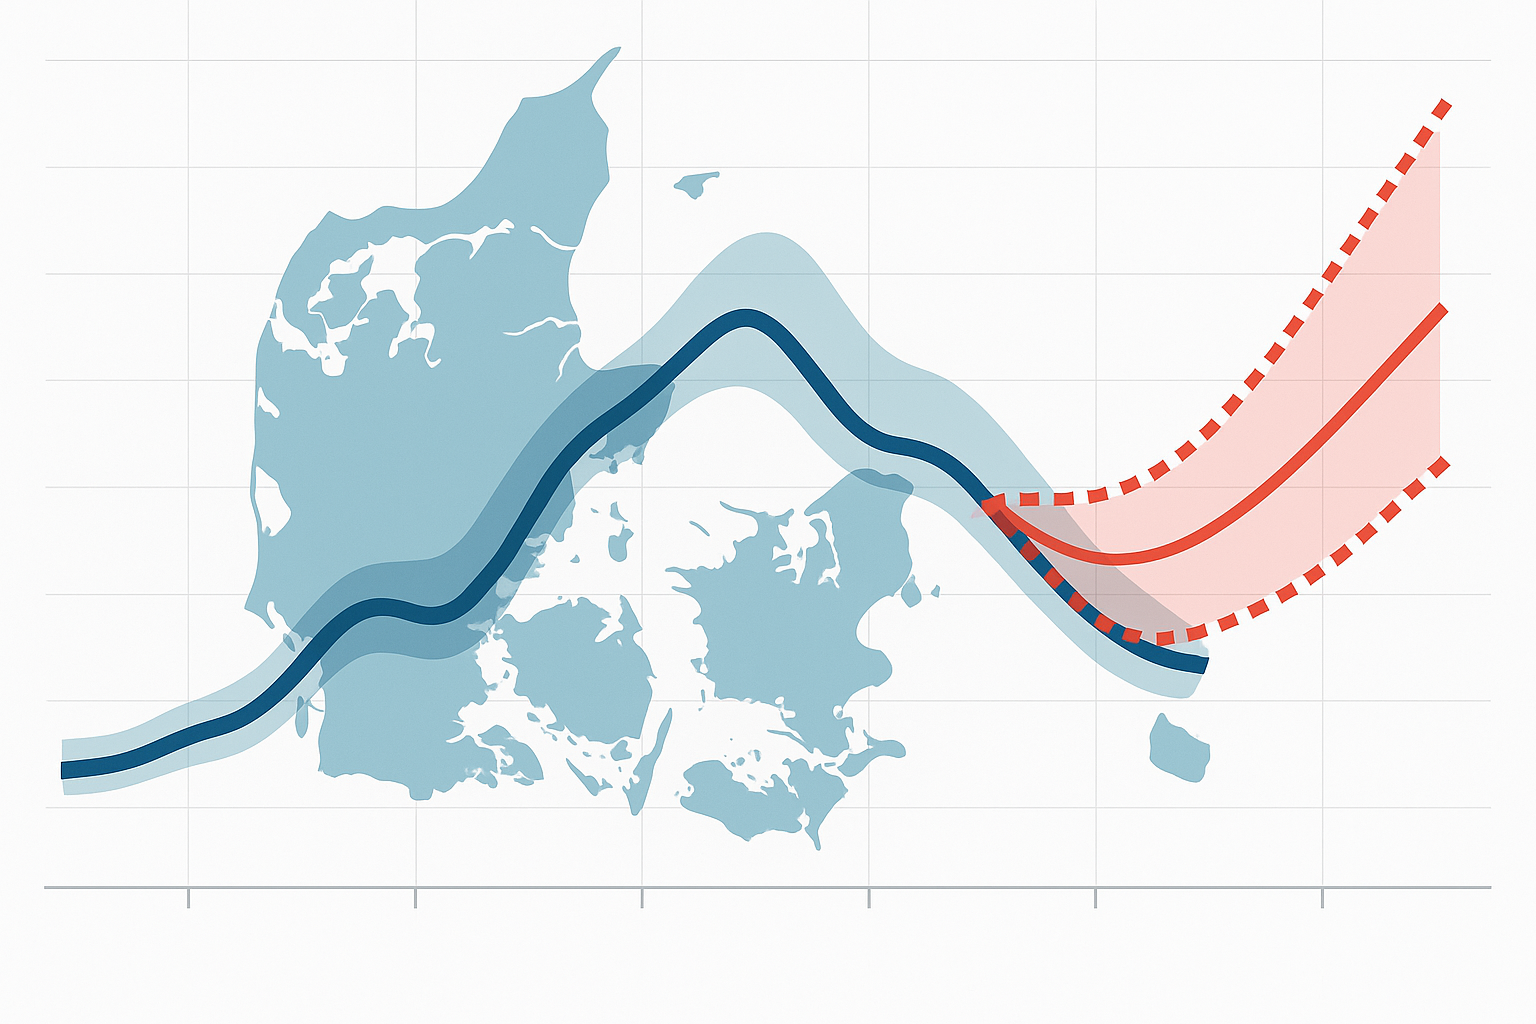
\includegraphics[width=0.9\textwidth]{fotos/forside.png} \\[2em]
\end{center}
\begin{center}
\fcolorbox{gray}{white}{
\parbox{0.8\textwidth}{
\centering
\textbf{Antal tegn (inkl. mellemrum): 32.000}
}}
\end{center}
\begin{center}
\textbf{Vejledere:} \\
Bjarne Taulo Sørensen \\
\end{center}

\newpage

\tableofcontents

\pagenumbering{arabic}
\setcounter{page}{1}
\newpage

\section{Introduktion}\label{introduktion}

Arbejdsløshedstal er en central indikator for et lands økonomiske
tilstand og udvikling. De påvirker både den enkelte borger og den
nationale økonomi og indgår som en væsentlig faktor i politiske og
økonomiske beslutningsprocesser. I takt med øget datatilgængelighed og
forbedrede statistiske værktøjer er det blevet muligt at analysere og
forudsige sådanne udviklingstræk med større præcision.

Denne opgave undersøger udviklingen i arbejdsløsheden i Danmark i
perioden 2007 til 2019 -- opdelt på køn og region. Datagrundlaget består
af ti tidsserier, én for hver kombination af fem regioner og to køn. Det
giver mulighed for at analysere både regionale forskelle og
kønsspecifikke mønstre i arbejdsløsheden.

Med udgangspunkt i klassiske tidsseriemodeller, ARIMA, ETS og en simpel
benchmarkmodel (Seasonal Naive), undersøges, hvordan arbejdsløsheden har
udviklet sig, og hvordan den kan fremskrives. Undervejs vurderes
modellernes egnethed med fokus på præcision og residualstruktur, og der
anvendes teknikker som STL-dekomposition og transformation af data.
Målet er ikke blot at forudsige udviklingen i 2020, men også at vurdere,
hvor godt klassiske modeller formår at håndtere forskellene mellem
regioner og køn.

\section{Problemformulering}\label{problemformulering}

Hvordan kan klassiske tidsseriemodeller anvendes til at analysere og
forudsige udviklingen i arbejdsløsheden i Danmark, fordelt på region og
køn?

For at besvare dette spørgsmål undersøges følgende delspørgsmål:

\begin{enumerate}
\def\labelenumi{\arabic{enumi}.}
\item
  Hvordan varierer arbejdsløshedens udvikling og sæsonmønstre på tværs
  af regioner og køn, og hvordan kan disse identificeres gennem
  eksplorativ dataanalyse og dekomposition?
\item
  Hvordan performer modellerne ARIMA, ETS og Seasonal Naive i forhold
  til hinanden, når det gælder præcision, residualstruktur og
  prognoseegenskaber?
\item
  Hvilke modeller er bedst egnede til at fremskrive
  arbejdsløshedstallene for 2020, og hvordan varierer usikkerheden på
  tværs af serier?
\end{enumerate}

\subsection{Afgrænsning}\label{afgruxe6nsning}

Analysen baserer sig udelukkende på de udleverede arbejdsløshedstal for
perioden januar 2007 til december 2019 og anvender ingen eksterne
forklaringsvariable såsom COVID-19, økonomiske indikatorer eller
politiske reformer. Dette valg er truffet for at isolere og vurdere
forecasting-modellernes metodiske egenskaber. Fokus er dermed på
reproducerbar, statistisk modellering -- ikke på årsagsforklaring eller
samfundsøkonomisk fortolkning.

\subsubsection{Anvendelse af
AI-værktøj}\label{anvendelse-af-ai-vuxe6rktuxf8j}

ChatGPT (GPT-4o) er anvendt som støtteværktøj i forbindelse med
idéudvikling, sproglig formulering og udformning af enkelte kodestumper.
Værktøjet er kun brugt til tekniske og sproglige formål -- al analyse,
fortolkning og konklusion er udarbejdet selvstændigt af gruppens
medlemmer.

\subsection{Definitioner/forkortelser}\label{definitionerforkortelser}

Nedenfor er en oversigt over centrale begreber og forkortelser, som
anvendes i opgaven:

\begin{itemize}
\tightlist
\item
  \textbf{ARIMA}: AutoRegressive Integrated Moving Average
\item
  \textbf{ETS}: Exponential Smoothing State Space Model
\item
  \textbf{SNAÏVE}: Seasonal Naive
\item
  \textbf{RMSE}: Root Mean Squared Error
\item
  \textbf{MAPE}: Mean Absolute Percentage Error
\item
  \textbf{STL}: Seasonal-Trend decomposition using Loess
\item
  \textbf{CV}: Cross-validation
\end{itemize}

\subsection{Struktur}\label{struktur}

Opgavens struktur følger en klassisk tilgang til tidsserieanalyse og er
inddelt i fem faser. Først gennemføres en eksplorativ dataanalyse med
fokus på mønstre og variationer i arbejdsløsheden fordelt på region og
køn. Dernæst estimeres tre modeller (ARIMA, ETS og Seasonal Naive) for
hver tidsserie. I tredje fase valideres modellerne gennem
krydsvalidering og residualanalyse. Herefter foretages fremskrivninger
for 2020, og til sidst sammenlignes og konkluderes der på tværs af
modeller og dataserier.

\section{Data og forberedelse}\label{data-og-forberedelse}

Analysen bygger på månedlige arbejdsløshedstal fra Danmark i perioden
januar 2007 til december 2019. Data er opdelt efter køn og region,
hvilket giver ti separate tidsserier. Datasættet er udleveret i et
forbehandlet tsibble-format med tydeligt definerede indeks- og
nøglevariabler, og nedenfor indlæses datasættet:

\begin{verbatim}
# A tsibble: 6 x 4 [1M]
# Key:       kon, region [1]
  kon     region             yearmonth svalue
  <fct>   <fct>                  <mth>  <dbl>
1 Kvinder Region Hovedstaden  2007 Jan   2.26
2 Kvinder Region Hovedstaden  2007 Feb   2.19
3 Kvinder Region Hovedstaden  2007 Mar   2.09
4 Kvinder Region Hovedstaden  2007 Apr   1.97
5 Kvinder Region Hovedstaden  2007 May   1.99
6 Kvinder Region Hovedstaden  2007 Jun   1.93
\end{verbatim}

\section{Eksplorativ dataanalyse
(EDA)}\label{eksplorativ-dataanalyse-eda}

Formålet med dette afsnit er at skabe et overblik over datasættets
struktur forud for modelleringen. Ved hjælp af visualiseringer,
deskriptive statistikker og STL-dekomposition undersøges
arbejdsløshedens udvikling på tværs af regioner og køn i perioden 2007
til 2019. Analysen afdækker overordnede tendenser, sæsonmønstre og
forskelle i niveau og variation. Resultaterne danner det metodiske
fundament for det videre modelarbejde.

\subsection{Visualisering af udvikling og
mønstre}\label{visualisering-af-udvikling-og-muxf8nstre}

I dette afsnit undersøges, hvordan arbejdsløsheden har udviklet sig over
tid -- med fokus på tendenser, sæsonvariationer og forskelle mellem
regioner og køn. Formålet er at identificere mønstre, som kan guide valg
af modeller i den videre analyse.

\subsubsection{Udvikling over tid}\label{udvikling-over-tid}

I de følgende figurer undersøges udviklingen i arbejdsløsheden over tid.
Til at begynde med anvendes den oprindelige skala for at give et
lettilgængeligt overblik (Figur 1). Fra Figur 2 og frem benyttes en
log-transformation for at stabilisere variationen i serierne, især
blandt mænd, og for at sikre sammenlignelighed i videre modellering og
forecast.

\pandocbounded{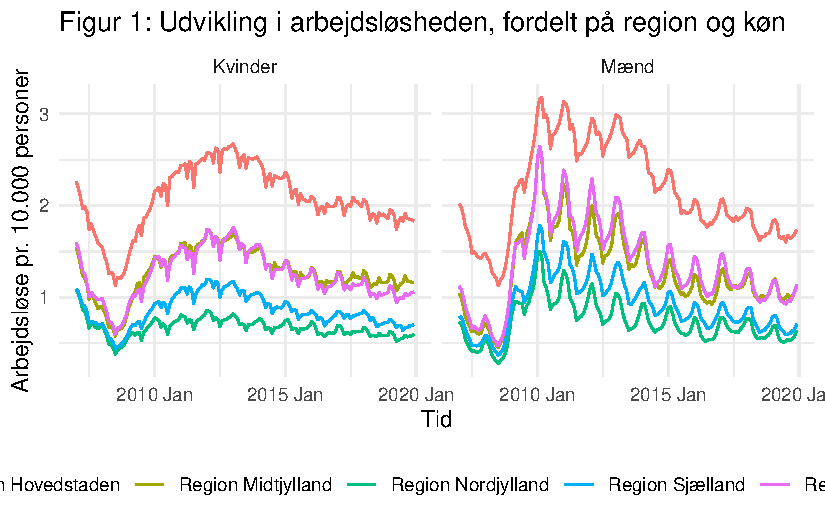
\includegraphics[keepaspectratio]{130625_Forecasting_files/figure-pdf/figur 1-1.pdf}}

Ovenstående figur viser den månedlige arbejdsløshed blandt mænd og
kvinder i de fem danske regioner fra 2007 til 2019. Der fremgår et
tydeligt sæsonmønster med højere ledighed i vintermånederne og lavere i
sommerperioden. Niveauet varierer regionalt, hvor Region Hovedstaden
typisk ligger højest og Nordjylland lavest. Samlet ses en faldende
tendens efter finanskrisen.

\pandocbounded{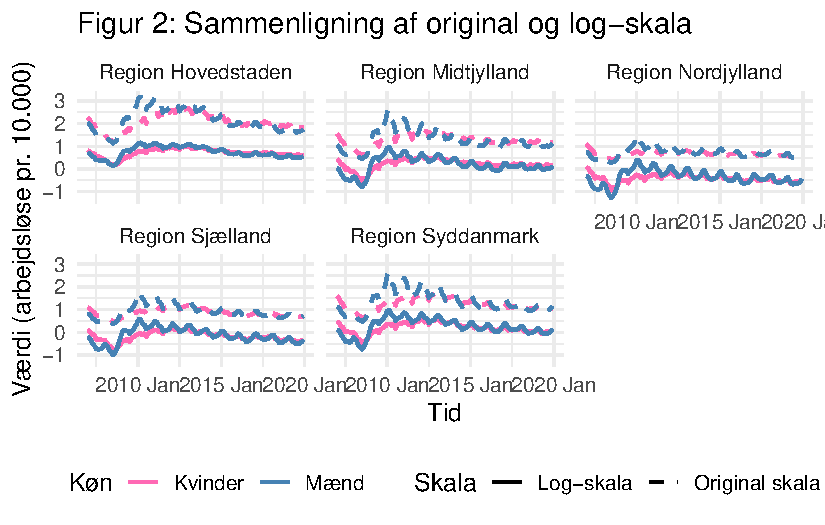
\includegraphics[keepaspectratio]{130625_Forecasting_files/figure-pdf/figur 2-1.pdf}}

Figur 2 viser, hvordan log-transformeringen dæmper udsvingene, særligt i
serier med højt niveau og stor variation, som det ses blandt mænd. Denne
transformation gør det lettere at sammenligne udviklingen på tværs af
regioner og køn og sikrer en mere stabil varians i det videre
analysearbejde. Derfor anvendes den log-transformerede version
fremadrettet i analysen.

\subsubsection{Sæsonmønstre}\label{suxe6sonmuxf8nstre}

Med log-transformerede data som fundament undersøges nu sæsonmønstrene i
arbejdsløsheden nærmere. Gennem sæsonplots og subserieplots vurderes,
hvordan arbejdsløsheden typisk varierer over året -- og hvordan dette
adskiller sig mellem mænd og kvinder samt på tværs af regioner.

\pandocbounded{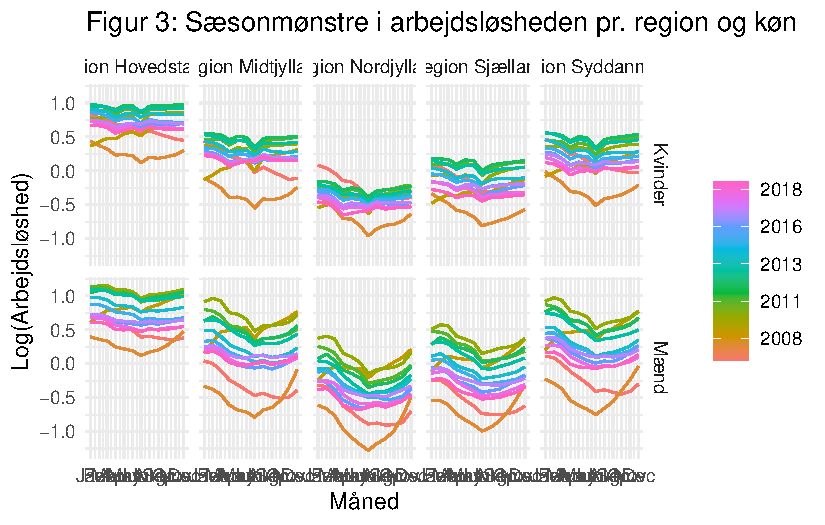
\includegraphics[keepaspectratio]{130625_Forecasting_files/figure-pdf/figur 3-1.pdf}}

Figur 3 viser sæsonmønstre i arbejdsløsheden pr. region og køn
(log-transformeret). Hver farve repræsenterer et år, og linjerne viser
en tydelig sæsonrytme med høj ledighed i årets begyndelse og lav i
sommermånederne. Mænd udviser generelt større sæsonudsving end kvinder.
Niveauet er højest i Region Hovedstaden og lavest i Nordjylland og
Sjælland. Negative log-værdier forekommer, hvor arbejdsløsheden ligger
under 1 pr. 10.000.

\pandocbounded{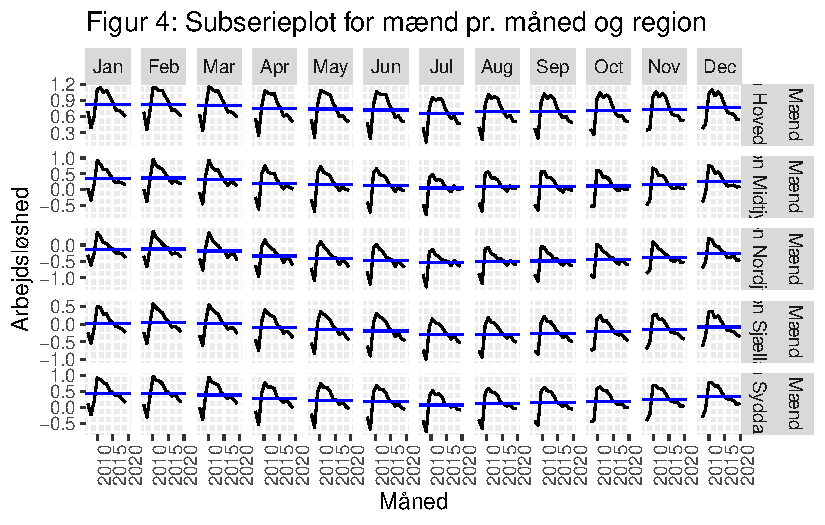
\includegraphics[keepaspectratio]{130625_Forecasting_files/figure-pdf/figur 4-1.pdf}}

Figur 4 viser subserieplottet for arbejdsløshedens udvikling for mænd
pr. måned og region. Hver celle viser forløbet for en specifik måned
over årene, med sorte linjer for de enkelte år og blå linjer for
gennemsnit. Ledigheden topper typisk i årets første måneder og falder
hen over sommeren. Mænd udviser generelt større sæsonudsving og højere
variation mellem år, især i vinterhalvåret.

\pandocbounded{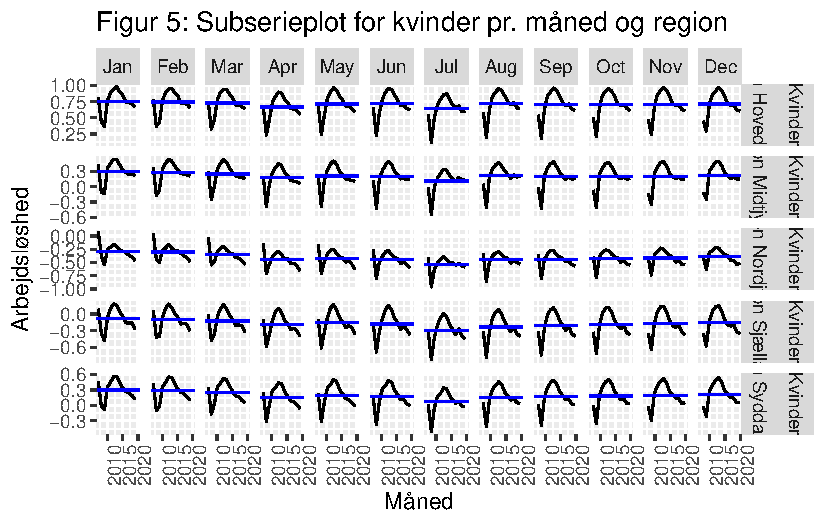
\includegraphics[keepaspectratio]{130625_Forecasting_files/figure-pdf/figur 5-1.pdf}}

Sammenlignet med mænd viser kvinder tilsvarende sæsonmønstre med højere
ledighed i årets begyndelse og lavere i sommermånederne. Udsvingene er
dog mindre markante, og variationen mellem år er mindre tydelig.
Mønstret fremstår mere stabilt og jævnt fordelt på tværs af regioner,
hvilket tyder på lavere volatilitet i kvindernes arbejdsløshed.

Udover sæsonmæssige udsving varierer arbejdsløsheden betydeligt på tværs
af både geografi og køn. Dette undersøges nærmere i de følgende
visualiseringer.

For at underbygge disse visuelle indsigter med konkrete tal, præsenteres
i næste afsnit deskriptive statistikker. De giver en numerisk
opsummering af centrale mål som gennemsnit, variation og ekstreme
værdier og bidrager til at identificere særligt stabile eller volatile
grupper, der kan kræve særlig opmærksomhed i den videre analyse.

\subsection{Deskriptive statistikker}\label{deskriptive-statistikker}

De foregående visualiseringer viste klare forskelle i arbejdsløshedens
niveau, variation og sæsonmønstre på tværs af regioner og køn (Figur
1--5). For at supplere disse observationer med en kvantitativ
opsummering præsenteres i Tabel 1 centrale deskriptive mål: gennemsnit,
standardafvigelse, minimum og maksimum. Tabellen giver et hurtigt
overblik over niveau og variation og fremhæver for eksempel Nordjylland
som en stabil region, særligt blandt kvinder, mens andre kombinationer
viser højere udsving.

\begin{longtable}[t]{llrrrr}
\caption{Deskriptiv statistik per region og køn}\\
\toprule
\cellcolor[HTML]{f0f0f0}{\textbf{region}} & \cellcolor[HTML]{f0f0f0}{\textbf{kon}} & \cellcolor[HTML]{f0f0f0}{\textbf{Gennemsnit}} & \cellcolor[HTML]{f0f0f0}{\textbf{Standardafvigelse}} & \cellcolor[HTML]{f0f0f0}{\textbf{Minimum}} & \cellcolor[HTML]{f0f0f0}{\textbf{Maksimum}}\\
\midrule
Region Hovedstaden & Kvinder & 2.07 & 0.36 & 1.13 & 2.67\\
Region Hovedstaden & Mænd & 2.17 & 0.52 & 1.13 & 3.18\\
Region Midtjylland & Kvinder & 1.27 & 0.25 & 0.58 & 1.72\\
Region Midtjylland & Mænd & 1.29 & 0.44 & 0.45 & 2.62\\
Region Nordjylland & Kvinder & 0.67 & 0.10 & 0.38 & 1.09\\
\addlinespace
Region Nordjylland & Mænd & 0.74 & 0.23 & 0.28 & 1.50\\
Region Sjælland & Kvinder & 0.86 & 0.17 & 0.45 & 1.20\\
Region Sjælland & Mænd & 0.92 & 0.30 & 0.37 & 1.78\\
Region Syddanmark & Kvinder & 1.24 & 0.26 & 0.60 & 1.76\\
Region Syddanmark & Mænd & 1.37 & 0.47 & 0.47 & 2.65\\
\bottomrule
\end{longtable}

\subsubsection{Features}\label{features}

Selvom deskriptive statistikker giver et første indtryk af variation og
niveau, indfanger de ikke strukturelle træk som trend, sæsonmønstre og
stationaritet. For at kvantificere disse egenskaber beregnes en række
såkaldte features ved hjælp af ved hjælp af funktionen features() fra
feasts-pakken (Hyndman \& Athanasopoulos, 2021, kap. 4).

Tabel 2 præsenterer udvalgte mål, der beskriver centrale træk ved
serierne og uddyber de visuelle indsigter fra Figur 1--5. Den
bagvedliggende kode, herunder brugen af features()-funktionen og
indlæsning af dataobjektet feature\_table.rds, er dokumenteret i Bilag
X.

\begin{longtable}[t]{llrrrrrr}
\caption{Deskriptiv statistik per region og køn}\\
\toprule
\cellcolor[HTML]{f0f0f0}{\textbf{kon}} & \cellcolor[HTML]{f0f0f0}{\textbf{region}} & \cellcolor[HTML]{f0f0f0}{\textbf{acf1}} & \cellcolor[HTML]{f0f0f0}{\textbf{seasonal\_strength\_year}} & \cellcolor[HTML]{f0f0f0}{\textbf{var\_tiled\_mean}} & \cellcolor[HTML]{f0f0f0}{\textbf{shift\_level\_max}} & \cellcolor[HTML]{f0f0f0}{\textbf{ndiffs}} & \cellcolor[HTML]{f0f0f0}{\textbf{trend\_strength}}\\
\midrule
Kvinder & Region Hovedstaden & 0.97 & 0.65 & 0.97 & 0.38 & 1 & 0.99\\
Kvinder & Region Midtjylland & 0.96 & 0.72 & 0.92 & 0.54 & 1 & 0.98\\
Kvinder & Region Nordjylland & 0.89 & 0.87 & 0.73 & 0.47 & 0 & 0.97\\
Kvinder & Region Sjælland & 0.96 & 0.81 & 0.92 & 0.43 & 1 & 0.99\\
Kvinder & Region Syddanmark & 0.96 & 0.83 & 0.91 & 0.45 & 1 & 0.99\\
\addlinespace
Mænd & Region Hovedstaden & 0.98 & 0.81 & 0.98 & 0.58 & 1 & 0.99\\
Mænd & Region Midtjylland & 0.98 & 0.84 & 0.93 & 1.05 & 0 & 0.98\\
Mænd & Region Nordjylland & 0.96 & 0.91 & 0.80 & 0.89 & 0 & 0.97\\
Mænd & Region Sjælland & 0.97 & 0.92 & 0.90 & 0.80 & 1 & 0.99\\
Mænd & Region Syddanmark & 0.98 & 0.88 & 0.91 & 0.96 & 1 & 0.98\\
\bottomrule
\end{longtable}

De kvantitative mål i Tabel 2 supplerer og styrker tolkningerne fra
Figur 1 til 5. I det følgende fremhæves de mest centrale mønstre med
fokus på fem analytiske temaer: autokorrelation, sæsonmønstre, variation
og skift, stationaritet og trend.

\textbf{Autokorrelation}

Variablen acf1 måler korttidsafhængighed, det vil sige, hvor stærkt
observationer i serien er knyttet til deres nære fortid. Værdierne
ligger generelt højt (typisk mellem 0,96 og 0,98), hvilket indikerer en
glidende udvikling uden pludselige udsving. Dette stemmer overens med de
jævne bevægelser og stabile tendenser, som blev observeret i Figur 1 og
Figur 2.

\textbf{Sæsonmønstre}

Styrken af årlige sæsonmønstre, målt med seasonal\_strength\_year,
varierer på tværs af grupper. Mænd udviser generelt mere udtalte
sæsonudsving end kvinder. For eksempel har mænd i Nordjylland og
Sjælland værdier på henholdsvis 0,91 og 0,92. Det svarer til de tydelige
sæsonrytmer vist i Figur 3, Figur 4 og Figur 5. I modsætning hertil har
kvinder i Region Hovedstaden en lavere værdi på 0,65, hvilket indikerer
en mere stabil sæsonprofil.

\textbf{Variation og skift}

Målet var\_tiled\_mean afspejler graden af variation inden for
afgrænsede perioder. Kvinder i Nordjylland har den laveste værdi (0,73),
hvilket viser en forholdsvis stabil udvikling over tid. Dette
understøttes af de glatte kurver i Figur 5. Variablen shift\_level\_max
måler derimod pludselige niveauskift. Mænd i Midtjylland udviser den
højeste værdi (1,05), hvilket sandsynligvis relaterer sig til reaktioner
på finanskrisen og kan ses i de kraftige fald i arbejdsløsheden i Figur
1 og Figur 2.

\textbf{Stationaritet}

Antallet af nødvendige differensieringer (ndiffs) angiver, hvorvidt en
serie er stationær. De fleste serier kræver én differens, men enkelte,
herunder kvinder i Nordjylland og mænd i både Midtjylland og
Nordjylland, har værdi 0. Dette indikerer, at de allerede er stationære
uden transformation, hvilket også kommer til udtryk i deres stabile
forløb i Figur 3 og Figur 5.

\textbf{Trend}

Variablen trend\_strength måler graden af trendstruktur i serien.
Værdierne ligger generelt meget højt (typisk 0,97 til 0,99), hvilket
bekræfter tydelige underliggende tendenser i arbejdsløsheden. Det gælder
især Region Hovedstaden, hvor niveauet er højt, og udviklingen over tid
er markant, som det fremgår af Figur 1 og Figur 2.

Samlet set bidrager funktionerne i Tabel 2 til at kvantificere og
validere de mønstre, der tidligere blev identificeret visuelt.
Autokorrelation, sæsonvariation og trendstruktur fremstår som
gennemgående karakteristika i alle serier, men med klare forskelle
mellem køn og regioner. Resultaterne danner et vigtigt grundlag for valg
af modeller og videre analyse.

\subsection{STL-dekomposition}\label{stl-dekomposition}

STL-dekomposition anvendes for at undersøge de strukturelle komponenter
i arbejdsløshedsserierne. Metoden opdeler tidsserierne i tre dele:
trend, sæson og remainder, hvilket giver indblik i, hvor stor en del af
variationen der skyldes henholdsvis langsigtet udvikling,
tilbagevendende mønstre eller kortsigtede udsving (Hyndman og
Athanasopoulos, 2021). Dekompositionen er udført separat for mænd og
kvinder i hver region, og resultaterne vises i figur 6 og 7.

\pandocbounded{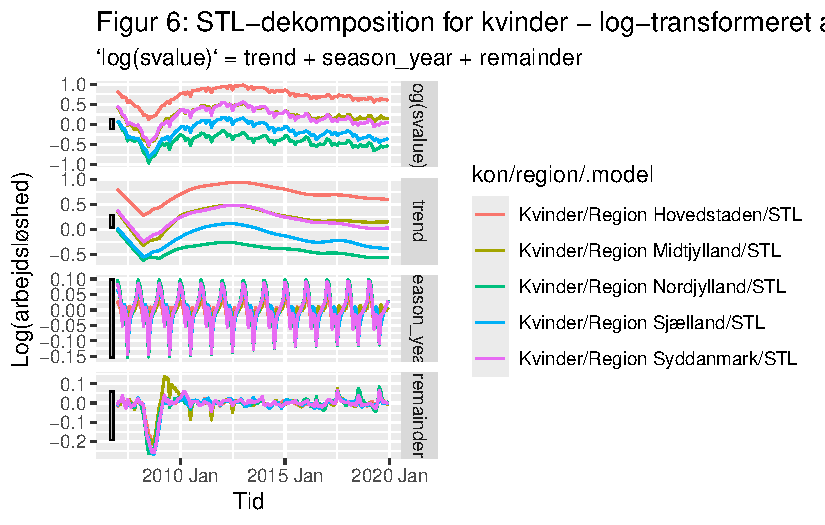
\includegraphics[keepaspectratio]{130625_Forecasting_files/figure-pdf/figur 6-1.pdf}}

Figur 6 viser STL-dekompositionen for kvinder i de fem danske regioner.
Der ses tydelige sæsonmønstre med tilbagevendende lavpunkter i
sommermånederne og højere ledighed i vinterhalvåret. Trends varierer
mellem regionerne: Region Hovedstaden udviser generelt højere ledighed,
mens Nordjylland og Sjælland ligger lavere. Residualerne ligger stabilt
omkring nul, hvilket indikerer, at modellen formår at fange de
dominerende strukturer i data.

\pandocbounded{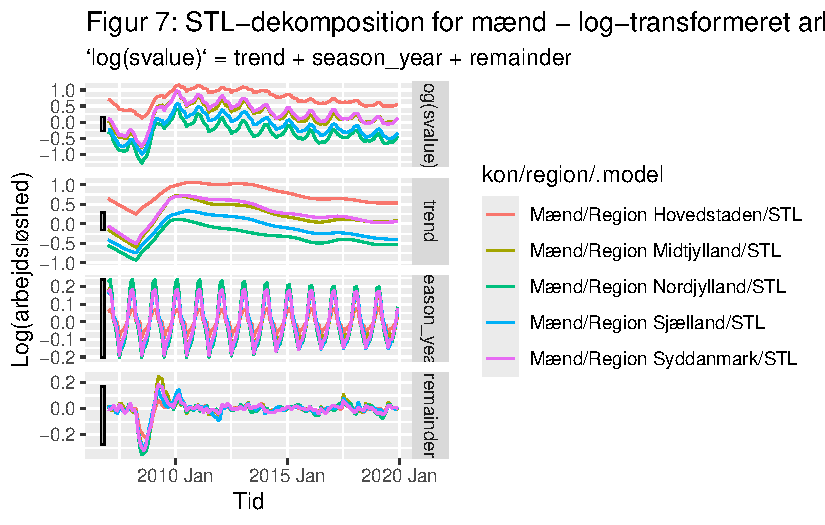
\includegraphics[keepaspectratio]{130625_Forecasting_files/figure-pdf/unnamed-chunk-2-1.pdf}}

Figur 7 viser tilsvarende dekomposition for mænd. Her ses en tilsvarende
stærk sæsonkomponent, men med mere markante udsving og højere
ledighedsniveauer -- især efter finanskrisen. Trends følger samme
overordnede forløb som for kvinder, men afvigelserne er større. Dette
bekræfter tidligere observationer om højere volatilitet i mænds
ledighed. Residualkomponenten er mere varierende, hvilket kan indikere,
at nogle udsving ikke fanges fuldt ud af modellen.

Disse observationer fra STL-dekompositionen bekræfter, at både trend og
sæsonmønstre varierer betydeligt på tværs af serierne. Det understreger
behovet for modeller, der kan tilpasses hver series struktur, hvilket
vil blive præsenteret i det følgende afsnit.

\section{Modelvalg}\label{modelvalg}

I dette afsnit estimeres og sammenlignes tre klassiske modeltyper,
ARIMA, ETS og benchmarkmodellen SNaive, for hver tidsserie (region ×
køn). Hver modeltype har forskellige antagelser og fordele og kan fange
forskellige karakteristika i data, såsom trend, sæson og
autokorrelation. Modelvalget foretages automatisk for hver serie via
fable-pakken, og resultaterne anvendes i den efterfølgende validering og
forecast.

\subsection{Valgte modeltyper}\label{valgte-modeltyper}

\textbf{ARIMA (AutoRegressive Integrated Moving Average)}\\
ARIMA-modeller anvendes til at modellere tidsserier med autokorrelation
og ikke-stationaritet. De kombinerer autoregressive (AR) led, differens
(I) for at opnå stationaritet, og glidende gennemsnit (MA) led til at
modellere fejl. Ved at inkludere sæsonkomponenter (SARIMA) kan modellen
håndtere årligt gentagende mønstre. ARIMA er særligt velegnet til serier
med langsigtede trends og strukturelle skift, hvor tidligere værdier har
stor indflydelse på den nuværende tilstand (Hyndman \& Athanasopoulos,
2021, kap. 9).

\textbf{ETS (Exponential Smoothing State Space Model)}\\
ETS-modeller benytter eksponentiel glatning til at vægte nyere
observationer højere og beskriver tidsserier ud fra tre elementer: fejl,
trend og sæson. Hver komponent kan være additiv eller multiplicativ
afhængigt af dataens karakter. ETS egner sig godt til serier med
tydelige strukturer og sæsonrytmer, især når der ikke er behov for at
modellere autokorrelation direkte (Hyndman \& Athanasopoulos, 2021, kap.
8).

\textbf{SNAÏVE (Seasonal Naive)}\\
SNaive er en enkel benchmarkmodel, der baserer hvert forecast på den
tilsvarende værdi fra samme sæson i den foregående periode. Modellen
fanger sæsonmønstre, men tager ikke højde for trend eller afhængighed i
data. Den anvendes til at vurdere, om mere komplekse modeller giver en
mærkbart bedre forecast-præcision (Hyndman \& Athanasopoulos, 2021, kap.
3 og 8).

\section{Modelvalidering}\label{modelvalidering}

Dette afsnit har til formål at sikre, at modellerne giver pålidelige
forecasts og ikke blot overtilpasser sig historiske data. Gennem
tidsserie-crossvalidering, fejlmålinger som RMSE og MAPE, samt
residualanalyse identificeres den bedst egnede model for hver serie,
baseret på forecastpræcision og modeladfærd.

\subsection{Splitning af datasættet}\label{splitning-af-datasuxe6ttet}

Vi starter med at splitte datasættet op i et træningssæt og et testsæt.
Testsættet er dataen fra hele 2019, som er det sidste år i det samlede
datasæt, og træningssættet er alt den forrige data fra 2007-2018.

\begin{Shaded}
\begin{Highlighting}[]
\NormalTok{train\_data }\OtherTok{\textless{}{-}}\NormalTok{ data }\SpecialCharTok{|\textgreater{}} \FunctionTok{filter\_index}\NormalTok{(. }\SpecialCharTok{\textasciitilde{}} \StringTok{"2018 Dec"}\NormalTok{)}
\NormalTok{test\_data  }\OtherTok{\textless{}{-}}\NormalTok{ data }\SpecialCharTok{|\textgreater{}} \FunctionTok{filter\_index}\NormalTok{(}\StringTok{"2019 Jan"} \SpecialCharTok{\textasciitilde{}} \StringTok{"2019 Dec"}\NormalTok{)}
\end{Highlighting}
\end{Shaded}

\subsection{Time-series
Cross-validation}\label{time-series-cross-validation}

Herunder udføres tidsserie-krydsvalidering udelukkende på træningsdataen
med et rullende vindue på 60 måneder. Vi anvender stretch\_tsibble() til
at generere flere trænings- og test-split, som forskydes én måned ad
gangen. Tre modeller evalueres: ARIMA, ETS og en sæsonbetonet naiv model
(SNaive) -- alle på log-transformerede data.

Forecastfejlene beregnes med accuracy(), og beregningerne køres
parallelt for hurtigere eksekvering. Resultaterne gemmes med
write\_rds() for reproducérbarhed.

\begin{Shaded}
\begin{Highlighting}[]
\CommentTok{\# plan(multisession)}

\CommentTok{\# cv\_data \textless{}{-} train\_data |\textgreater{}}
\CommentTok{\#   stretch\_tsibble(.init = 60, .step = 1)}

\CommentTok{\# cv\_models \textless{}{-} cv\_data |\textgreater{}}
\CommentTok{\#   model(}
\CommentTok{\#     ARIMA  = ARIMA(log(svalue)),}
\CommentTok{\#     ETS    = ETS(log(svalue)),}
\CommentTok{\#     SNaive = SNAIVE(log(svalue))}
\CommentTok{\#   )}

\CommentTok{\# write\_rds(cv\_models, "cv\_models.rds")}

\NormalTok{cv\_models }\OtherTok{\textless{}{-}} \FunctionTok{read\_rds}\NormalTok{(}\StringTok{"data/cv\_models.rds"}\NormalTok{)}

\NormalTok{cv\_accuracy }\OtherTok{\textless{}{-}}\NormalTok{ cv\_models }\SpecialCharTok{|\textgreater{}}
  \FunctionTok{accuracy}\NormalTok{()}

\CommentTok{\# plan(sequential)}
\end{Highlighting}
\end{Shaded}

\subsubsection{Valg af bedste model for hver tidsserie, baseret på
CV}\label{valg-af-bedste-model-for-hver-tidsserie-baseret-puxe5-cv}

Her identificeres den bedste model for hver kombination af køn og region
baseret på laveste RMSE. Ved at gruppere på kon og region og vælge
modellen med mindst fejl (slice\_min()), får vi én vinder pr. serie uden
ligestilling mellem modeller (with\_ties = FALSE). Dette gør det muligt
senere at bruge den bedste model til forecast for hver delserie.

\begin{Shaded}
\begin{Highlighting}[]
\NormalTok{vinder\_cv }\OtherTok{\textless{}{-}}\NormalTok{ cv\_accuracy }\SpecialCharTok{|\textgreater{}}
  \FunctionTok{group\_by}\NormalTok{(kon, region) }\SpecialCharTok{|\textgreater{}}
  \FunctionTok{slice\_min}\NormalTok{(RMSE, }\AttributeTok{n =} \DecValTok{1}\NormalTok{, }\AttributeTok{with\_ties =} \ConstantTok{FALSE}\NormalTok{) }\SpecialCharTok{|\textgreater{}}
  \FunctionTok{ungroup}\NormalTok{()}

\NormalTok{vinder\_cv }\SpecialCharTok{|\textgreater{}} \FunctionTok{select}\NormalTok{(kon, region, .model)}
\end{Highlighting}
\end{Shaded}

\begin{verbatim}
# A tibble: 10 x 3
   kon     region             .model
   <fct>   <fct>              <chr> 
 1 Kvinder Region Hovedstaden ETS   
 2 Kvinder Region Midtjylland ARIMA 
 3 Kvinder Region Nordjylland ARIMA 
 4 Kvinder Region Sjælland    ARIMA 
 5 Kvinder Region Syddanmark  ARIMA 
 6 Mænd    Region Hovedstaden ARIMA 
 7 Mænd    Region Midtjylland ARIMA 
 8 Mænd    Region Nordjylland ARIMA 
 9 Mænd    Region Sjælland    ARIMA 
10 Mænd    Region Syddanmark  ARIMA 
\end{verbatim}

Resultaterne viser, at ARIMA-modellen klarer sig bedst i 9 ud af 10
tidsserier. Den eneste undtagelse er kvinder i Region Hovedstaden, hvor
en ETS-model giver lavest RMSE. Dette tyder på, at ARIMA generelt formår
at tilpasse sig strukturen i dataserierne bedre, hvilket ofte skyldes
modellens fleksibilitet i forhold til både trend og sæson. Den ene
ETS-vinder indikerer dog, at i nogle tilfælde kan eksponentiel glatning
være mere passende -- muligvis pga. mere stabil sæson uden kompleks
autokorrelation.

\subsection{Træning af vindermodel på hele datasættet og test på
2019-data}\label{truxe6ning-af-vindermodel-puxe5-hele-datasuxe6ttet-og-test-puxe5-2019-data}

\begin{Shaded}
\begin{Highlighting}[]
\NormalTok{model\_train }\OtherTok{\textless{}{-}}\NormalTok{ train\_data }\SpecialCharTok{|\textgreater{}}
  \FunctionTok{model}\NormalTok{(}
    \AttributeTok{ARIMA  =} \FunctionTok{ARIMA}\NormalTok{(}\FunctionTok{log}\NormalTok{(svalue)),}
    \AttributeTok{ETS    =} \FunctionTok{ETS}\NormalTok{(}\FunctionTok{log}\NormalTok{(svalue)),}
    \AttributeTok{SNaive =} \FunctionTok{SNAIVE}\NormalTok{(}\FunctionTok{log}\NormalTok{(svalue))}
\NormalTok{  )}

\NormalTok{train\_accuracy }\OtherTok{\textless{}{-}}\NormalTok{ model\_train }\SpecialCharTok{|\textgreater{}} 
  \FunctionTok{accuracy}\NormalTok{() }\SpecialCharTok{|\textgreater{}} 
  \FunctionTok{select}\NormalTok{(kon, region, .model, }\AttributeTok{RMSE\_tr =}\NormalTok{ RMSE, }\AttributeTok{MAPE\_tr =}\NormalTok{ MAPE)}

\NormalTok{forecast\_2019 }\OtherTok{\textless{}{-}}\NormalTok{ model\_train }\SpecialCharTok{|\textgreater{}}
  \FunctionTok{forecast}\NormalTok{(}\AttributeTok{h =} \StringTok{"12 months"}\NormalTok{) }\SpecialCharTok{|\textgreater{}}
  \FunctionTok{inner\_join}\NormalTok{(vinder\_cv,                      }
             \AttributeTok{by =} \FunctionTok{c}\NormalTok{(}\StringTok{"kon"}\NormalTok{, }\StringTok{"region"}\NormalTok{, }\StringTok{".model"}\NormalTok{))}
\end{Highlighting}
\end{Shaded}

Her gentrænes alle tre modeller på hele træningsperioden fra 2010 til
2018. Derefter laves et 12-måneders forecast for 2019, som svarer til
testperioden. Ved at forecaste alle modeller og derefter filtrere til
den tidligere udpegede vinder (inner\_join() med vinder\_cv), sikrer vi,
at den bedste model anvendes til hver serie i den endelige evaluering.

Her sammenlignes trænings- og testfejl for hver serie ved at kombinere
dem i én tabel (train\_vs\_test). Dette giver overblik over, hvorvidt
modellerne generaliserer godt --- altså om performance på testdata
svarer til performance på træningsdata.

\subsection{Sammenligning af trænings- og
testscore}\label{sammenligning-af-truxe6nings--og-testscore}

\begin{Shaded}
\begin{Highlighting}[]
\NormalTok{test\_accuracy }\OtherTok{\textless{}{-}}\NormalTok{ forecast\_2019 }\SpecialCharTok{|\textgreater{}}
  \FunctionTok{accuracy}\NormalTok{(test\_data) }\SpecialCharTok{|\textgreater{}}
  \FunctionTok{select}\NormalTok{(kon, region, .model, RMSE, MAPE)}

\NormalTok{train\_vs\_test }\OtherTok{\textless{}{-}} \FunctionTok{left\_join}\NormalTok{(train\_accuracy, test\_accuracy,}
                           \AttributeTok{by =} \FunctionTok{c}\NormalTok{(}\StringTok{"kon"}\NormalTok{, }\StringTok{"region"}\NormalTok{, }\StringTok{".model"}\NormalTok{))}

\NormalTok{train\_vs\_test }\OtherTok{\textless{}{-}}\NormalTok{ train\_vs\_test }\SpecialCharTok{|\textgreater{}} 
  \FunctionTok{filter}\NormalTok{(}\SpecialCharTok{!}\FunctionTok{is.na}\NormalTok{(RMSE)) }\SpecialCharTok{|\textgreater{}}
  \FunctionTok{relocate}\NormalTok{(RMSE, }\AttributeTok{.after =}\NormalTok{ RMSE\_tr)}

\NormalTok{train\_vs\_test}
\end{Highlighting}
\end{Shaded}

\begin{verbatim}
# A tibble: 10 x 7
   kon     region             .model RMSE_tr   RMSE MAPE_tr  MAPE
   <fct>   <fct>              <chr>    <dbl>  <dbl>   <dbl> <dbl>
 1 Kvinder Region Hovedstaden ETS     0.0434 0.0398    1.68  1.82
 2 Kvinder Region Midtjylland ARIMA   0.0290 0.0436    1.70  3.43
 3 Kvinder Region Nordjylland ARIMA   0.0133 0.0122    1.46  1.72
 4 Kvinder Region Sjælland    ARIMA   0.0156 0.0280    1.28  2.88
 5 Kvinder Region Syddanmark  ARIMA   0.0238 0.0236    1.41  1.85
 6 Mænd    Region Hovedstaden ARIMA   0.0383 0.0784    1.26  4.13
 7 Mænd    Region Midtjylland ARIMA   0.0503 0.0193    2.41  1.52
 8 Mænd    Region Nordjylland ARIMA   0.0296 0.0140    2.49  2.00
 9 Mænd    Region Sjælland    ARIMA   0.0289 0.0153    1.94  1.85
10 Mænd    Region Syddanmark  ARIMA   0.0464 0.0846    2.12  6.86
\end{verbatim}

Sammenligningen af trænings- og testfejl viser, at modellerne generelt
præsterer fornuftigt, men med variation. I flere serier er fejlene på
testdata lavere end på træningsdata (f.eks. mænd i Region Midtjylland og
Nordjylland). Omvendt ser vi enkelte serier med markant højere testfejl
(f.eks. mænd i Region Hovedstaden og Syddanmark), hvilket kan indikere
overfitting eller uforudsete udsving i 2019.

\subsubsection{Analyse af residualer og
autokorrelation}\label{analyse-af-residualer-og-autokorrelation}

Der er herunder udvalgt 3 tidsserier med forskellige situationer ift.
forskellen på trænings- og testscore, som der er blevet dykket længere
ned i med gg\_tsresiduals.

\begin{Shaded}
\begin{Highlighting}[]
\NormalTok{model\_train }\SpecialCharTok{|\textgreater{}}
  \FunctionTok{filter}\NormalTok{(kon }\SpecialCharTok{==} \StringTok{"Mænd"}\NormalTok{, region }\SpecialCharTok{==} \StringTok{"Region Syddanmark"}\NormalTok{) }\SpecialCharTok{|\textgreater{}}
  \FunctionTok{select}\NormalTok{(ARIMA) }\SpecialCharTok{|\textgreater{}} 
  \FunctionTok{gg\_tsresiduals}\NormalTok{()}
\end{Highlighting}
\end{Shaded}

\pandocbounded{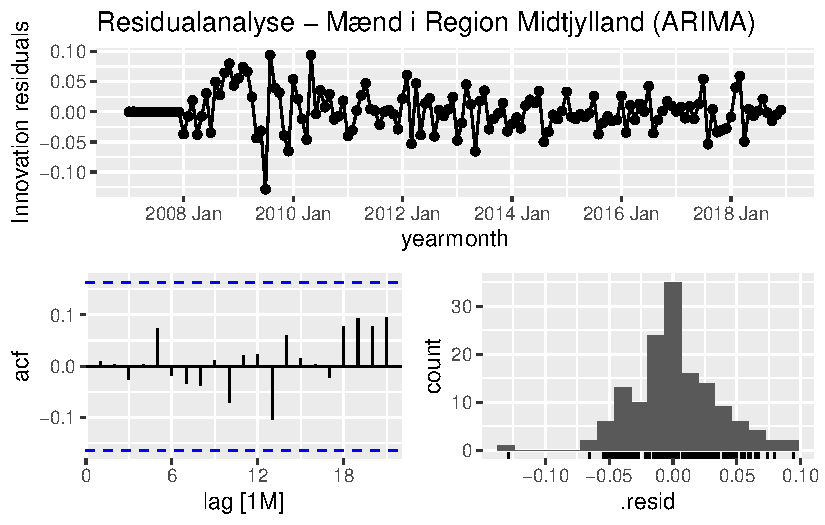
\includegraphics[keepaspectratio]{130625_Forecasting_files/figure-pdf/unnamed-chunk-8-1.pdf}}

Der er kigget nærmere på tidsserien for mænd i region Syddanmark, da den
har relativt høj test-RMSE ift. de andre og høj forskel på trænings- og
testscore.

Residualerne ser ud til at være nogenlunde centreret omkring nul, men
der er enkelte ekstreme udsving (outliers), særligt i 2009 og 2016.

ACF-plottet viser, at der ikke er signifikant autokorrelation i
residualerne --- alle ligger inden for konfidensgrænserne. Det er et
tegn på, at modellen har fanget den systematiske struktur i data.
Histogrammet indikerer en rimelig symmetrisk fordeling, men med lidt
tungere haler end en ideel normalfordeling.

Samlet set tyder residualanalysen på, at modellen er acceptabel, men de
ekstreme observationer og den relativt høje forecastfejl på testdata
(RMSE = 0.085) antyder, at modellen kan være følsom over for enkelte
udsving.

\begin{Shaded}
\begin{Highlighting}[]
\NormalTok{model\_train }\SpecialCharTok{|\textgreater{}}
  \FunctionTok{filter}\NormalTok{(kon }\SpecialCharTok{==} \StringTok{"Mænd"}\NormalTok{, region }\SpecialCharTok{==} \StringTok{"Region Midtjylland"}\NormalTok{) }\SpecialCharTok{|\textgreater{}}
  \FunctionTok{select}\NormalTok{(ARIMA) }\SpecialCharTok{|\textgreater{}} 
  \FunctionTok{gg\_tsresiduals}\NormalTok{()}
\end{Highlighting}
\end{Shaded}

\pandocbounded{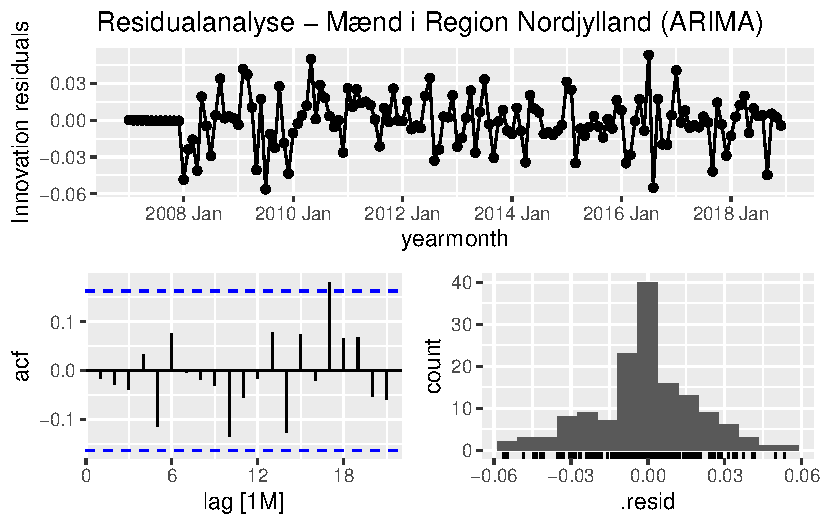
\includegraphics[keepaspectratio]{130625_Forecasting_files/figure-pdf/unnamed-chunk-9-1.pdf}}

Der er kigget nærmere på tidsserien for mænd i region Midtjylland, da
den har lav test-RMSE ift. trænings-RMSE.

Modellen ser ud til at have fanget strukturen i data rimeligt godt.
Residualerne er generelt centreret omkring nul, men enkelte større
afvigelser ses tidligt i serien.

ACF-plottet viser svag autokorrelation ved nogle højere lags, men ingen
værdier ligger tydeligt uden for konfidensgrænserne. Histogrammet viser
en nogenlunde symmetrisk fordeling med lette afvigelser fra normalitet.

Samlet set er der ikke tegn på systematiske fejl i residualerne. Det
stemmer godt overens med den relativt lave RMSE på testdata (RMSE =
0.019) sammenlignet med en højere træningsfejl (RMSE = 0.050), hvilket
tyder på, at modellen generaliserer bedre end forventet.

\begin{Shaded}
\begin{Highlighting}[]
\NormalTok{model\_train }\SpecialCharTok{|\textgreater{}}
  \FunctionTok{filter}\NormalTok{(kon }\SpecialCharTok{==} \StringTok{"Kvinder"}\NormalTok{, region }\SpecialCharTok{==} \StringTok{"Region Nordjylland"}\NormalTok{) }\SpecialCharTok{|\textgreater{}}
  \FunctionTok{select}\NormalTok{(ARIMA) }\SpecialCharTok{|\textgreater{}} 
  \FunctionTok{gg\_tsresiduals}\NormalTok{()}
\end{Highlighting}
\end{Shaded}

\pandocbounded{\includegraphics[keepaspectratio]{130625_Forecasting_files/figure-pdf/unnamed-chunk-10-1.pdf}}

Til sidst er der kigget nærmere på tidsserien for kvinder i region
Nordjylland, da den har lav test-RMSE og lav trænings-RMSE.

Residualerne er pænt centreret omkring nul og uden tydelige mønstre over
tid. Der ses enkelte udsving, men ingen systematiske afvigelser.

ACF-plottet viser lidt autokorrelation ved lag 17, men det virker
rimelig tilfældigt og ellers ligger værdierne inden for
konfidensgrænserne, hvilket tyder på, at modellen har fanget den
væsentlige struktur i data. Histogrammet viser en forholsvist symmetrisk
fordeling af residualerne.

Samlet set understøtter residualanalysen, at modellen er velfungerende
for denne serie. Det stemmer overens med en lav forecastfejl på testdata
(RMSE = 0.012) og indikerer, at modellen generaliserer stabilt.

\subsubsection{Ljung-tests for
tidsserier}\label{ljung-tests-for-tidsserier}

\begin{Shaded}
\begin{Highlighting}[]
\NormalTok{ljung\_box\_results }\OtherTok{\textless{}{-}}\NormalTok{ model\_train }\SpecialCharTok{|\textgreater{}} 
  \FunctionTok{augment}\NormalTok{() }\SpecialCharTok{|\textgreater{}}
  \FunctionTok{features}\NormalTok{(.innov, ljung\_box, }\AttributeTok{lag =} \DecValTok{24}\NormalTok{, }\AttributeTok{dof =} \DecValTok{3}\NormalTok{)}

\NormalTok{ljung\_box\_vindere }\OtherTok{\textless{}{-}}\NormalTok{ ljung\_box\_results }\SpecialCharTok{|\textgreater{}}
  \FunctionTok{inner\_join}\NormalTok{(vinder\_cv, }\AttributeTok{by =} \FunctionTok{c}\NormalTok{(}\StringTok{"kon"}\NormalTok{, }\StringTok{"region"}\NormalTok{, }\StringTok{".model"}\NormalTok{)) }\SpecialCharTok{|\textgreater{}} 
  \FunctionTok{select}\NormalTok{(}\DecValTok{1}\SpecialCharTok{:}\DecValTok{5}\NormalTok{)}
\end{Highlighting}
\end{Shaded}

For hver vinder-model er der udført en Ljung-Box test med 24 lags og 3
frihedsgrader for at vurdere, om residualerne er serielt uafhængige.

Resultaterne viser, at 9 ud af 10 modeller har høje p-værdier, hvilket
betyder, at vi ikke forkaster nulhypotesen om uafhængige residualer. Det
tyder på, at modellerne har fanget den væsentlige struktur i data.

Dog er der en klar undtagelse: ETS-modellen for kvinder i Region
Hovedstaden har en meget lav p-værdi, hvilket tyder på signifikant
autokorrelation i residualerne. Det skaber tvivl om modellens gyldighed
her og kunne indikere, at ARIMA muligvis havde været et bedre valg for
denne serie.

Samlet set tyder resultaterne på, at residualerne fra de fleste modeller
kan betragtes som hvid støj, hvilket er et centralt krav i vurderingen
af en god tidsseriemodel.

\section{Sammenligning af 2019 forudsigelser og
virkeligheden}\label{sammenligning-af-2019-forudsigelser-og-virkeligheden}

\begin{Shaded}
\begin{Highlighting}[]
\NormalTok{forecast\_vs\_actual }\OtherTok{\textless{}{-}}\NormalTok{ forecast\_2019 }\SpecialCharTok{|\textgreater{}}
  \FunctionTok{left\_join}\NormalTok{(}
\NormalTok{    test\_data }\SpecialCharTok{|\textgreater{}} \FunctionTok{select}\NormalTok{(kon, region, yearmonth, }\AttributeTok{actual =}\NormalTok{ svalue),}
    \AttributeTok{by =} \FunctionTok{c}\NormalTok{(}\StringTok{"kon"}\NormalTok{, }\StringTok{"region"}\NormalTok{, }\StringTok{"yearmonth"}\NormalTok{)}
\NormalTok{  )}

\NormalTok{forecast\_vs\_actual }\SpecialCharTok{|\textgreater{}}
  \FunctionTok{ggplot}\NormalTok{(}\FunctionTok{aes}\NormalTok{(}\AttributeTok{x =}\NormalTok{ yearmonth)) }\SpecialCharTok{+}
  \FunctionTok{geom\_line}\NormalTok{(}\FunctionTok{aes}\NormalTok{(}\AttributeTok{y =}\NormalTok{ actual), }\AttributeTok{color =} \StringTok{"black"}\NormalTok{, }\AttributeTok{size =} \FloatTok{0.9}\NormalTok{, }\AttributeTok{linetype =} \StringTok{"solid"}\NormalTok{) }\SpecialCharTok{+}
  \FunctionTok{geom\_line}\NormalTok{(}\FunctionTok{aes}\NormalTok{(}\AttributeTok{y =}\NormalTok{ .mean), }\AttributeTok{color =} \StringTok{"blue"}\NormalTok{, }\AttributeTok{size =} \FloatTok{0.9}\NormalTok{, }\AttributeTok{linetype =} \StringTok{"dashed"}\NormalTok{) }\SpecialCharTok{+}
  \FunctionTok{facet\_grid}\NormalTok{(region }\SpecialCharTok{\textasciitilde{}}\NormalTok{ kon, }\AttributeTok{scales =} \StringTok{"free\_y"}\NormalTok{) }\SpecialCharTok{+}
  \FunctionTok{labs}\NormalTok{(}
    \AttributeTok{title =} \StringTok{"Forecast vs. Faktiske værdier – 2019"}\NormalTok{,}
    \AttributeTok{y =} \StringTok{"Arbejdsløse pr. 10.000 personer"}\NormalTok{,}
    \AttributeTok{x =} \StringTok{"Tid"}\NormalTok{,}
    \AttributeTok{caption =} \StringTok{"Sort = Faktisk | Blå = Forecast"}
\NormalTok{  ) }\SpecialCharTok{+}
  \FunctionTok{theme\_minimal}\NormalTok{(}\AttributeTok{base\_size =} \DecValTok{13}\NormalTok{)}
\end{Highlighting}
\end{Shaded}

\pandocbounded{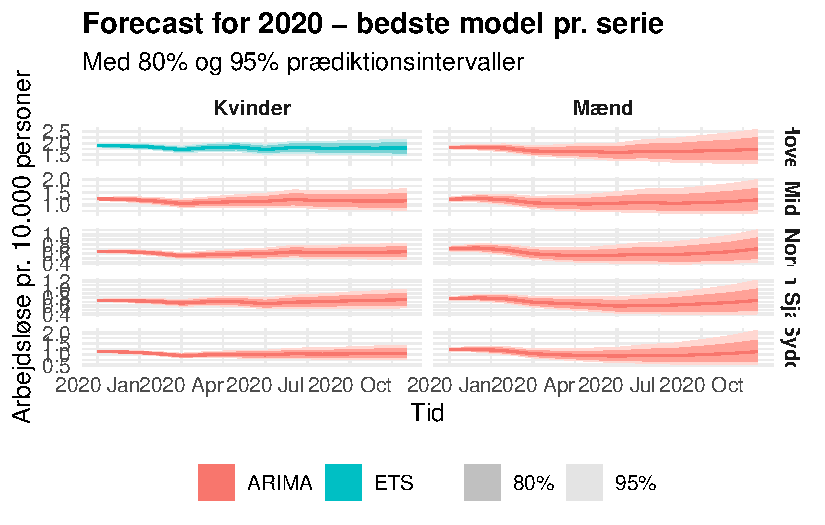
\includegraphics[keepaspectratio]{130625_Forecasting_files/figure-pdf/unnamed-chunk-12-1.pdf}}

Plottet viser en sammenligning mellem de faktiske observationer (sort)
og modellernes punktprognoser (blå) for 2019, opdelt på køn og region.
Generelt følger prognoserne udviklingen i de faktiske data tæt, hvilket
bekræfter, at modellerne har god forudsigelsesevne.

Særligt for mænd i Region Midtjylland og Nordjylland er der meget tæt
overensstemmelse. Derimod ses systematiske afvigelser for mænd i Region
Syddanmark og kvinder i Region Hovedstaden, hvor modellerne
undervurderer eller overvurderer udviklingen. Det stemmer overens med de
højere RMSE-værdier og residualanalyser for disse serier.

\section{Forecasting af 2020 for alle
tidsserier}\label{forecasting-af-2020-for-alle-tidsserier}

\begin{Shaded}
\begin{Highlighting}[]
\NormalTok{data\_train\_final }\OtherTok{\textless{}{-}}\NormalTok{ data}

\NormalTok{models\_final }\OtherTok{\textless{}{-}}\NormalTok{ data\_train\_final }\SpecialCharTok{|\textgreater{}} 
  \FunctionTok{model}\NormalTok{(}
    \AttributeTok{ARIMA  =} \FunctionTok{ARIMA}\NormalTok{(}\FunctionTok{log}\NormalTok{(svalue)),}
    \AttributeTok{ETS    =} \FunctionTok{ETS}\NormalTok{(}\FunctionTok{log}\NormalTok{(svalue)),}
    \AttributeTok{SNaive =} \FunctionTok{SNAIVE}\NormalTok{(}\FunctionTok{log}\NormalTok{(svalue))}
\NormalTok{  )}

\NormalTok{forecast\_2020 }\OtherTok{\textless{}{-}}\NormalTok{ models\_final }\SpecialCharTok{|\textgreater{}} 
  \FunctionTok{forecast}\NormalTok{(}\AttributeTok{h =} \StringTok{"12 months"}\NormalTok{) }\SpecialCharTok{|\textgreater{}} 
  \FunctionTok{inner\_join}\NormalTok{(vinder\_cv, }\AttributeTok{by =} \FunctionTok{c}\NormalTok{(}\StringTok{"kon"}\NormalTok{, }\StringTok{"region"}\NormalTok{, }\StringTok{".model"}\NormalTok{))}

\NormalTok{forecast\_2020 }\SpecialCharTok{|\textgreater{}} 
  \FunctionTok{autoplot}\NormalTok{(}\AttributeTok{level =} \FunctionTok{c}\NormalTok{(}\DecValTok{80}\NormalTok{, }\DecValTok{95}\NormalTok{)) }\SpecialCharTok{+}
  \FunctionTok{facet\_grid}\NormalTok{(region }\SpecialCharTok{\textasciitilde{}}\NormalTok{ kon, }\AttributeTok{scales =} \StringTok{"free\_y"}\NormalTok{) }\SpecialCharTok{+}
  \FunctionTok{labs}\NormalTok{(}
    \AttributeTok{title =} \StringTok{"Forecast for 2020 – bedste model pr. serie"}\NormalTok{,}
    \AttributeTok{subtitle =} \StringTok{"Med 80\% og 95\% prædiktionsintervaller"}\NormalTok{,}
    \AttributeTok{y =} \StringTok{"Arbejdsløse pr. 10.000 personer"}\NormalTok{,}
    \AttributeTok{x =} \StringTok{"Tid"}
\NormalTok{  ) }\SpecialCharTok{+}
  \FunctionTok{theme\_minimal}\NormalTok{(}\AttributeTok{base\_size =} \DecValTok{12}\NormalTok{) }\SpecialCharTok{+}
  \FunctionTok{theme}\NormalTok{(}
    \AttributeTok{legend.position =} \StringTok{"bottom"}\NormalTok{,}
    \AttributeTok{legend.title =} \FunctionTok{element\_blank}\NormalTok{(),}
    \AttributeTok{plot.title =} \FunctionTok{element\_text}\NormalTok{(}\AttributeTok{face =} \StringTok{"bold"}\NormalTok{),}
    \AttributeTok{strip.text =} \FunctionTok{element\_text}\NormalTok{(}\AttributeTok{face =} \StringTok{"bold"}\NormalTok{)}
\NormalTok{  )}
\end{Highlighting}
\end{Shaded}

\pandocbounded{\includegraphics[keepaspectratio]{130625_Forecasting_files/figure-pdf/unnamed-chunk-13-1.pdf}}

Plottet viser 12 måneders fremskrivning for 2020 baseret på den bedste
model pr. serie, suppleret med 80\% og 95\% prædiktionsintervaller. For
de fleste serier anvendes ARIMA (rød), mens ETS (turkis) kun bruges for
kvinder i Region Hovedstaden.

De fleste forecasts viser relativt stabile niveauer i arbejdsløsheden,
men for flere mandlige serier (især Region Syddanmark og Midtjylland)
ses en tydelig stigning og stigende usikkerhed hen over året -- hvilket
afspejles i de bredere konfidensbånd.

Visualiseringen illustrerer både det forventede niveau og usikkerheden i
prognoserne, og den bekræfter, at modellerne er i stand til at fange
forskelle mellem regioner og køn.

\section{Konsklusion}\label{konsklusion}

\newpage

\section{Kildeliste}\label{kildeliste}

Hyndman, R. J., \& Athanasopoulos, G. (2021). Forecasting: principles
and practice (3rd ed.). OTexts. https://otexts.com/fpp3/

OpenAI. (2025). ChatGPT (v.4o) {[}Large language model{]}.
https://chat.openai.com/

\newpage

\section{Bilagsoversigt}\label{bilagsoversigt}

\begin{itemize}
\tightlist
\item
  Bilag 1: Features
\end{itemize}




\end{document}
